% \chapter{Macro-commandes}
\section{Macro-commandes}

\subsection{Les différentes macros}%
\paragraph{}
Avant de pouvoir créer une macro \gls{vba} j'ai du apprendre les bases de ce langage et les outils utilisés. Pour cela je me suis aidé de certains sites internet tels que \url{http://www.excel-pratique.com}. J'ai finalement appris tout en créant ma première macro. 

En ce qui concerne les outils utilisés : j'utilisais Excel version 2007 sur Windows XP. La version d'Excel est important car des macros créés sous Excel 2007 ne peuvent pas forcément être lancées sur une version antérieure. 

Je vais maintenant vous parler des macros qui m'ont été demandées. Tout d'abord, il m'a été demandé de créer des macros afin d'automatiser des traitements effectués tous les jours, pour certains, par ma maître d'apprentissage. 

La première macro qui m'a été demandée consistait à calculer des statistiques sur les interventions effectuées par les techniciens. Cette macro a servi de feuille de contrôle des statistiques et des \gls{ri} transmis à la hotline.

Puis, j'ai dû créer une macro servant à éditer un fichier contenant des statistiques sur la productivité de chaque techniciens (cf. figure~\ref{prodDesTech} page~\pageref{prodDesTech}).
\begin{center}
  \begin{figure}[ht]
    \caption{\label{prodDesTech} Tableau de productivité des techniciens}
    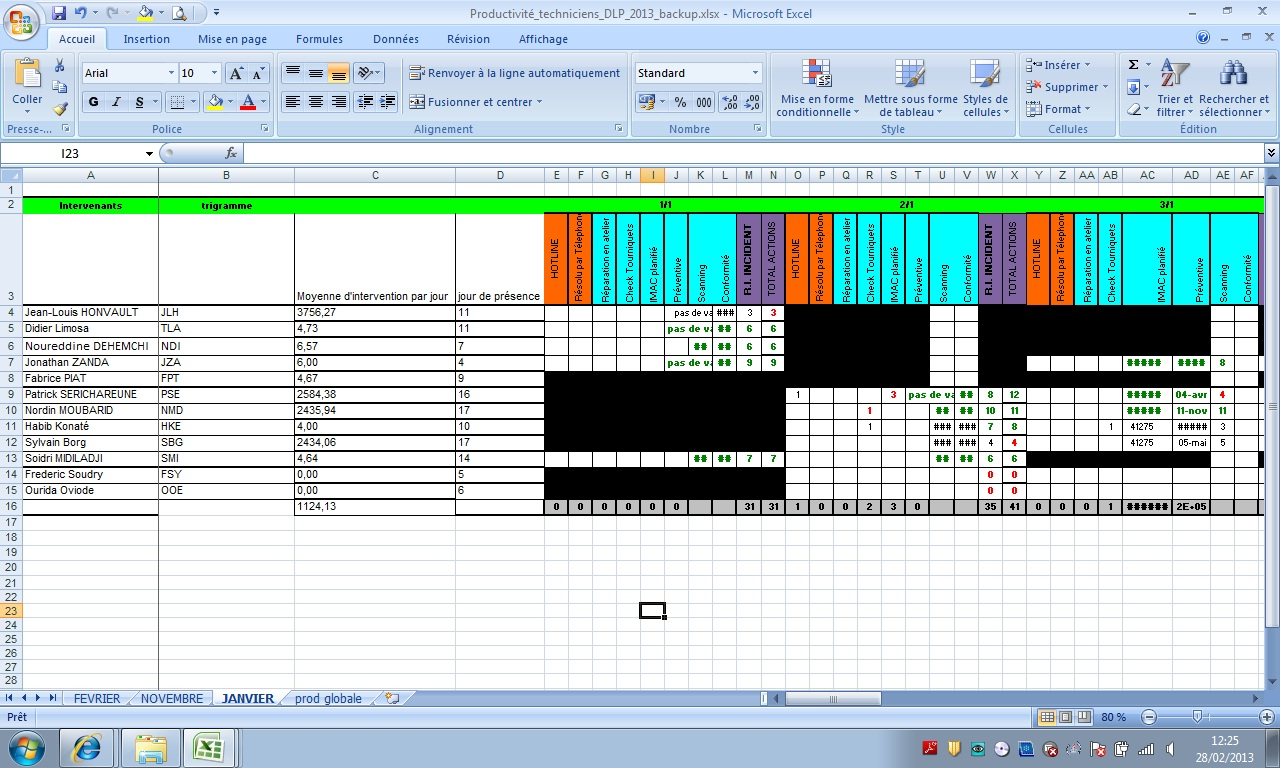
\includegraphics [width=1\textwidth]{images/prodDesTech.jpg}
  \end{figure}
\end{center}
\newacronym{sla}{SLA}{Service Level Agreement}
Ma troisième macro devait elle aussi servir à éditer un fichier déjà existant afin cette fois-ci d'établir un graphique sur le respect des \gls{sla} et des délais de manière plus globale.

Enfin, il m'a été demandé d'extraire automatiquement les listes des interventions résolues puis une deuxième liste pour les interventions en \gls{backlog} (cf. figure~\ref{listeResolu} page~\pageref{listeResolu}). et figure~\ref{listeBacklog} page~\pageref{listeBacklog}. 
Le fichier des interventions en \gls{backlog} doit absolument être édité et non pas recréé. Sinon, il perd tout son intérêt.
\begin{center}
  \begin{figure}[ht]
    \caption{\label{listeResolu} Listes des interventions résolues sur une période donnée}
    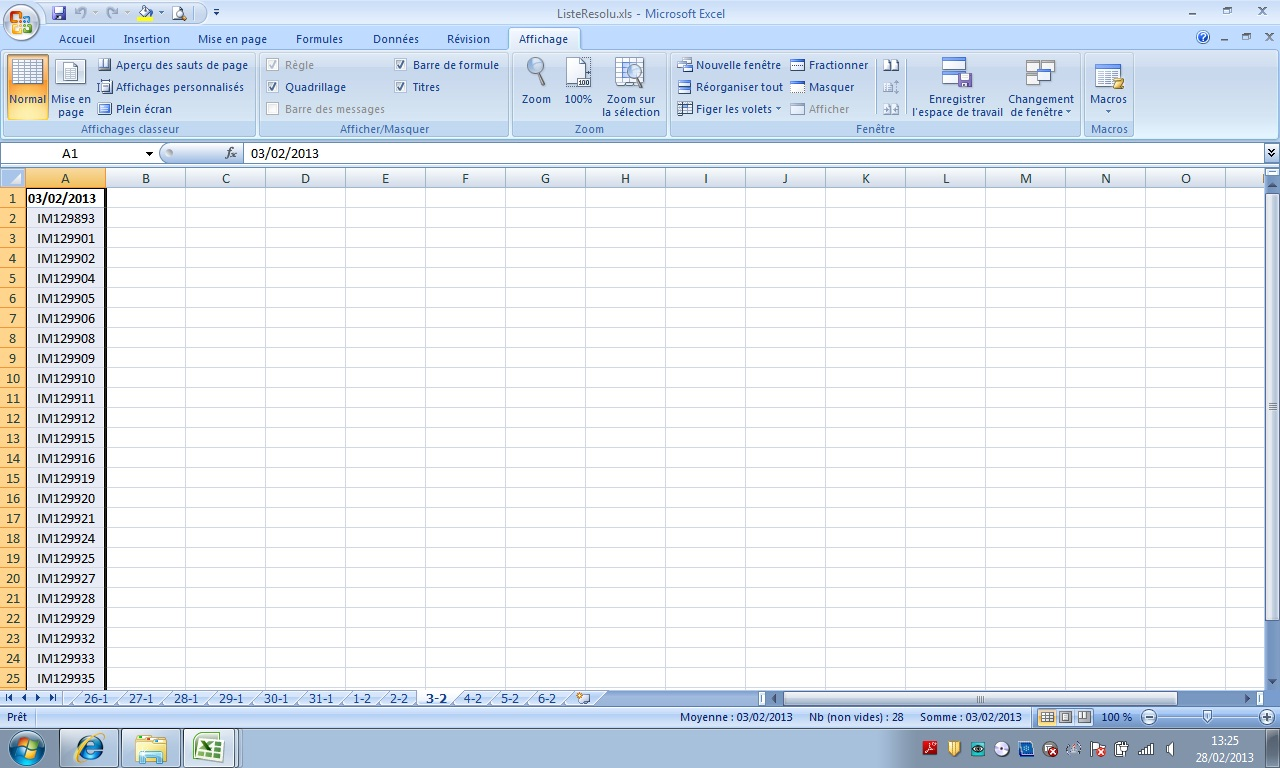
\includegraphics [width=1\textwidth]{images/listeResolu.jpg}
  \end{figure}
\end{center}
\begin{center}
  \begin{figure}[ht]
    \caption{\label{listeBacklog} Listes des interventions en backlog}
    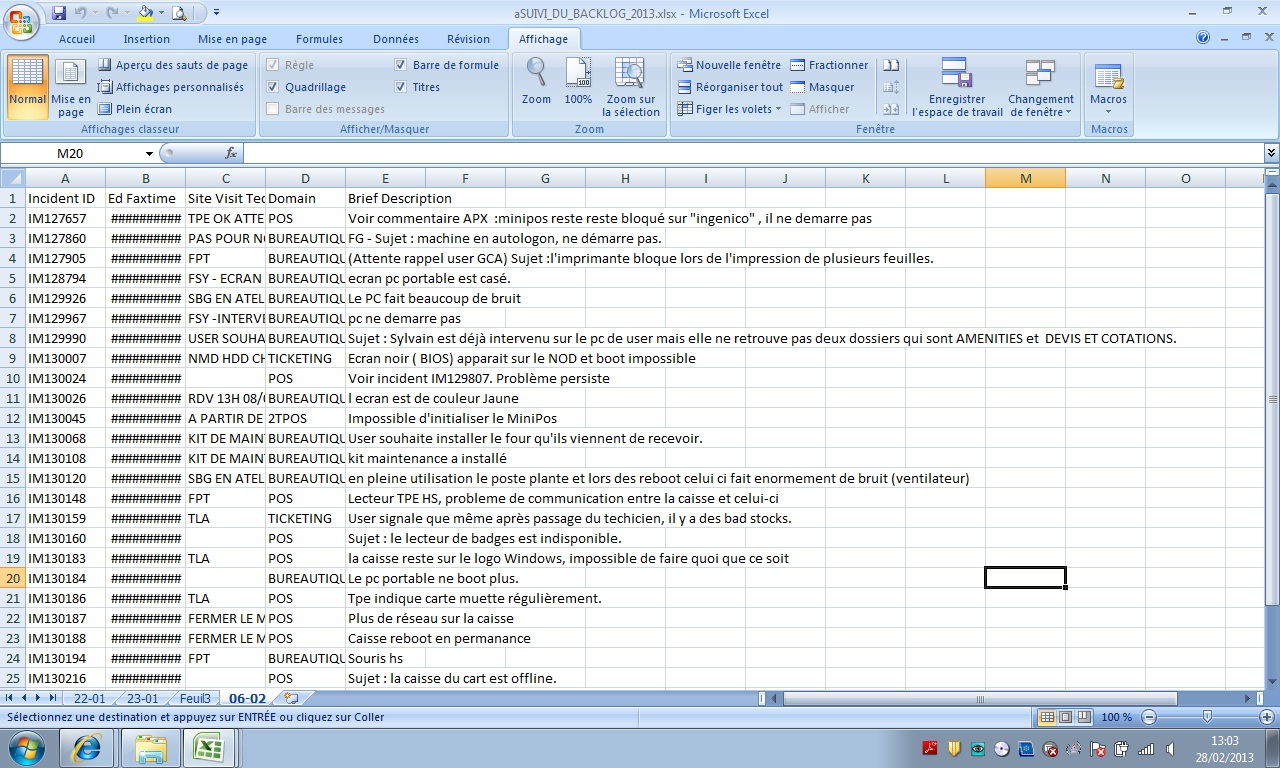
\includegraphics [width=1\textwidth]{images/listeBacklog.jpg}
  \end{figure}
\end{center}


\subsection{La conception}%
\paragraph{}
Je vais maintenant vous parler de tout ce qui concerne la conception de ces macros. Tout d'abord, les données extraites de \gls{sm7} pour établir les statistiques demandées n'étaient pas triées en fonction du destinataire de l'\gls{ot}. Il a donc fallu trier ces données avant de pouvoir les exploiter. Sur la photo~\ref{ExtractSM7} page~\pageref{ExtractSM7}, on remarque que dans la colonne BG correspondant au destinataire de l'\gls{ot}, il y a des noms d'autres services comme "Customer" qui s'occupe de la maintenance \foreignlanguage{english}{\gls{software}} du parc. Toutes les lignes n'étant pas adressées à notre service devaient être retirées. 
\begin{center}
  \begin{figure}[ht]
    \caption{\label{ExtractSM7} Extrait de données SM7}
    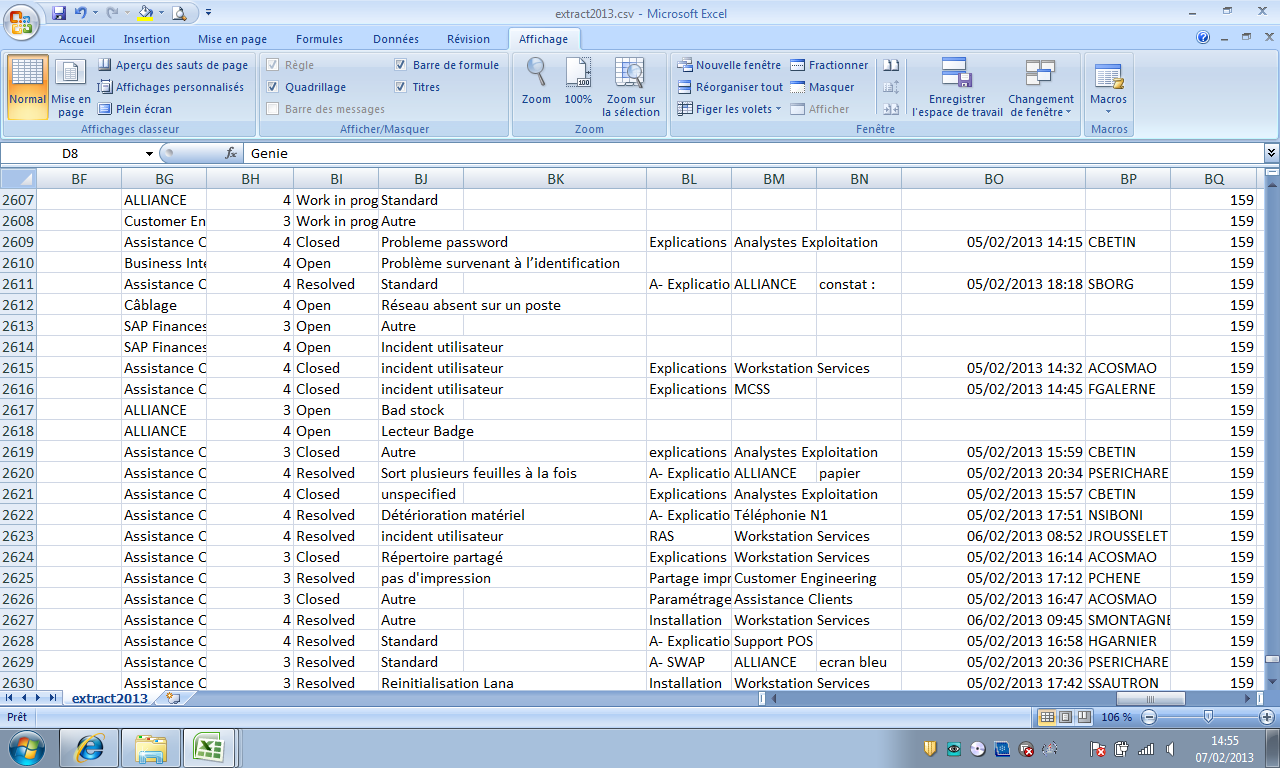
\includegraphics [width=1\textwidth]{images/ExtractSM7.png}
  \end{figure}
\end{center}

J'ai donc effectué un premier tri sur ces données en créant une nouvelle feuille Excel et en y copiant seulement les lignes voulues et les colonnes utilisées. Ce qui donne la figure~\ref{premierTrie} page~\pageref{premierTrie}.
\begin{center}
  \begin{figure}[ht]
    \caption{\label{premierTrie} Extrait de données SM7 après un premier trie}
    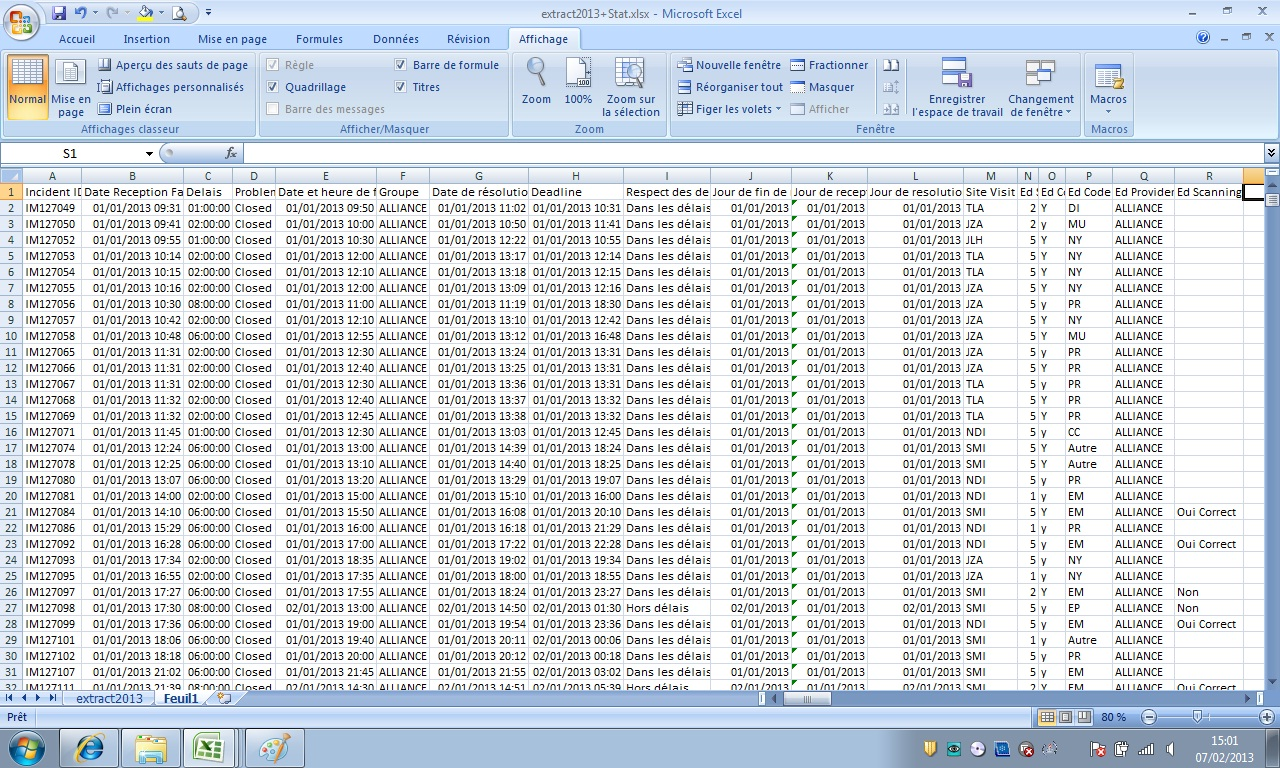
\includegraphics [width=1\textwidth]{images/premierTrie.jpg}
  \end{figure}
\end{center}
C'est donc sur cette feuille que vont se baser la plupart des macros que j'ai réalisé.

\paragraph{}
Une fois ce traitement effectué, j'ai utilisé ces données pour calculer des statistiques. J'ai commencé par créer la macro de "contrôle" mentionnée plus haut. J'ai utilisé des tableaux croisés dynamique et d'autres outils disponibles dans Excel pour arriver facilement à un résultat. 
Les tableaux et statistiques que je calcule sont stockés dans la même feuille que les données. Parmi les statistiques que je calcule, certaines seront copiées directement dans le fichier de productivité des techniciens. 

Le résultat de la macro de "contrôle" correspond aux images~\ref{premierCalculs} page~\pageref{premierCalculs}, \ref{deuxiemeTraitement} page~\pageref{deuxiemeTraitement} et \ref{troisiemeTraitement} page~\pageref{troisiemeTraitement}.
\begin{center}
  \begin{figure}[ht]
    \caption{\label{premierCalculs} Première partie du résultat de la macro "contrôle"}
    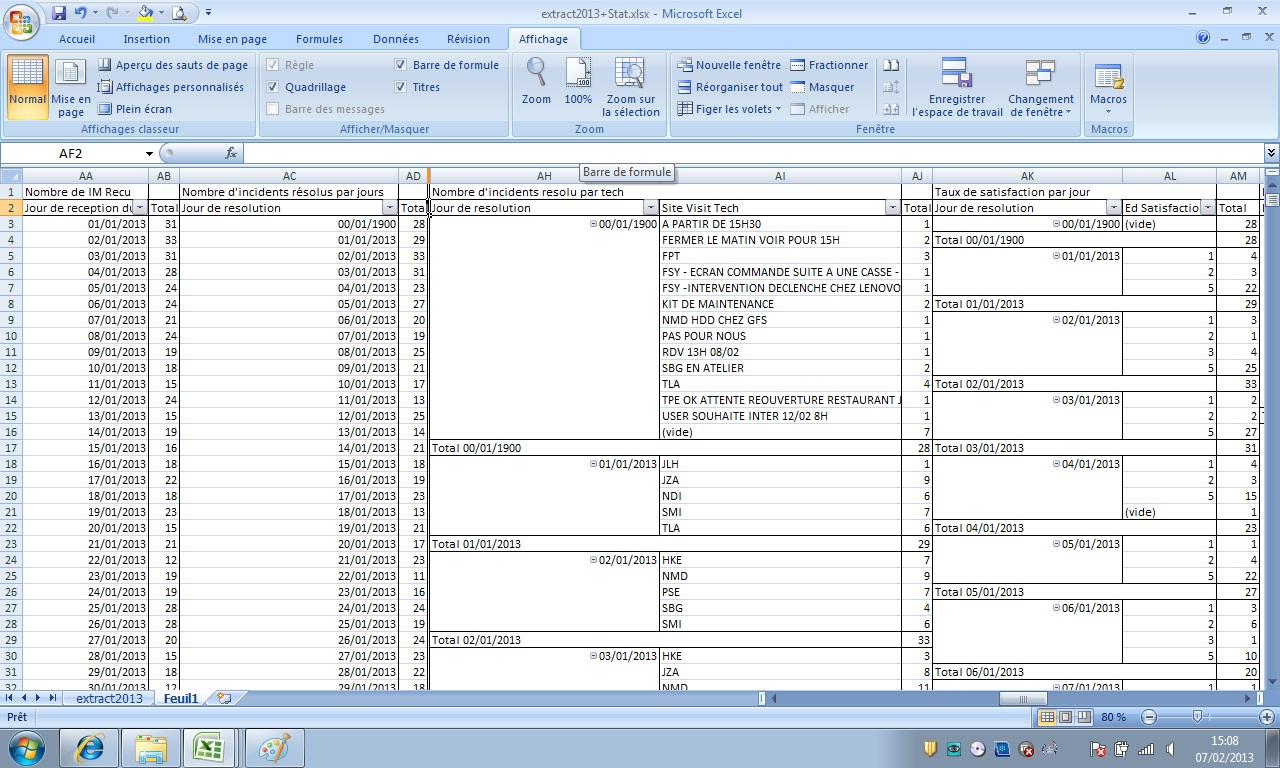
\includegraphics [width=1\textwidth]{images/premierCalculs.jpg}
  \end{figure}
\end{center}
\begin{center}
  \begin{figure}[ht]
    \caption{\label{deuxiemeTraitement} Deuxième partie du résultat de la macro "contrôle"}
    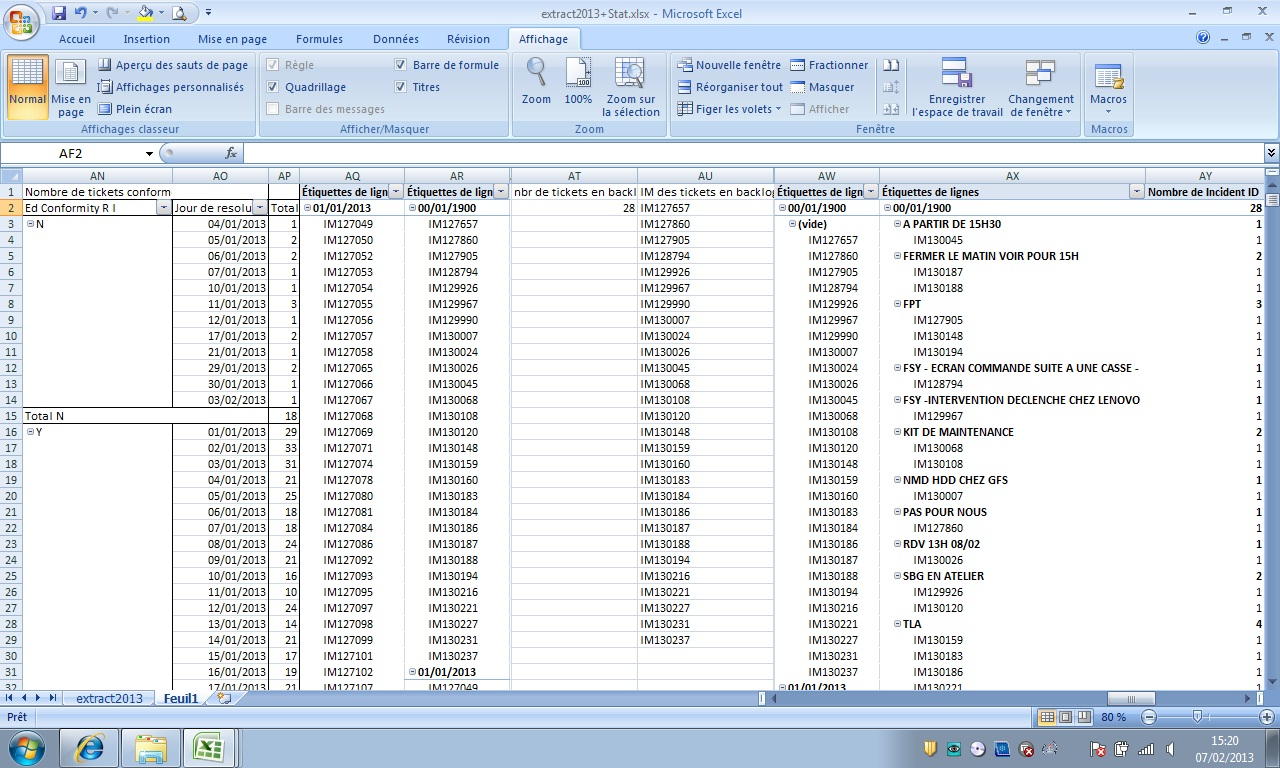
\includegraphics [width=1\textwidth]{images/deuxiemeTraitement.jpg}
  \end{figure}
\end{center}
\begin{center}
  \begin{figure}[ht]
    \caption{\label{troisiemeTraitement} Troisième partie du résultat de la macro "contrôle"}
    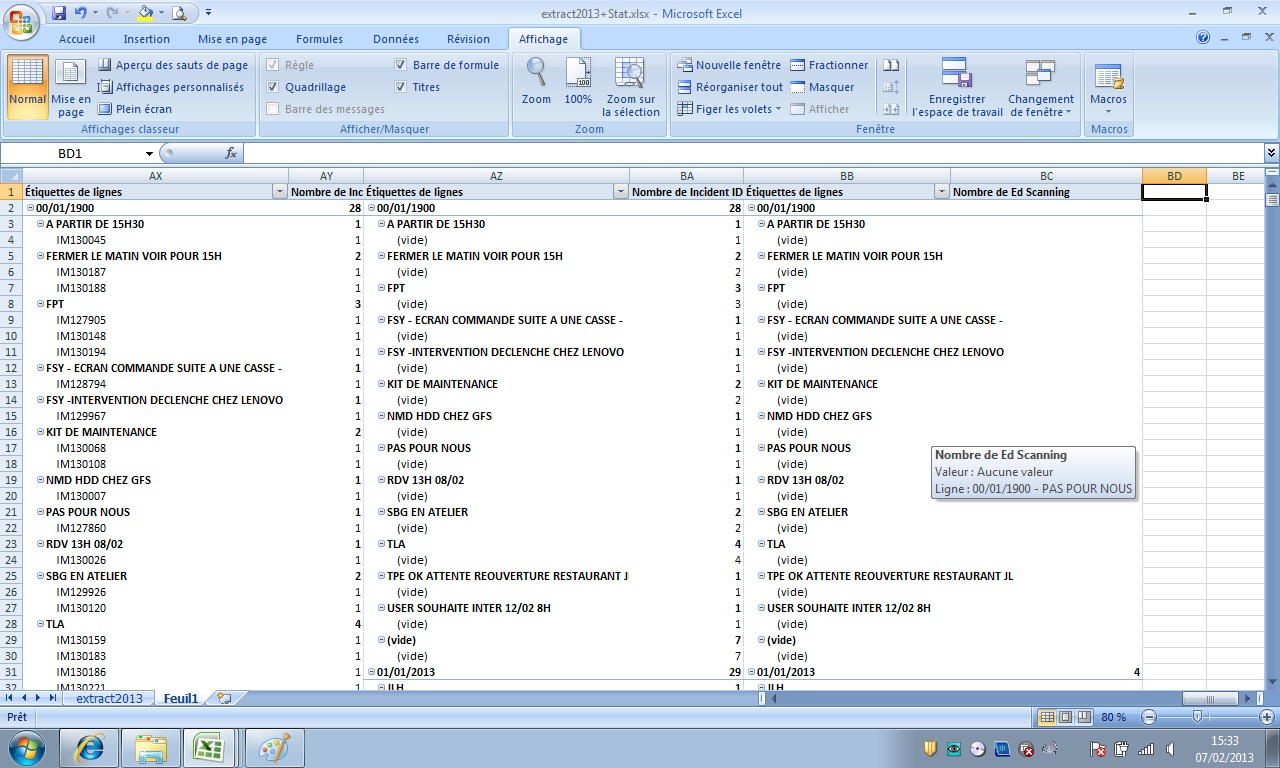
\includegraphics [width=1\textwidth]{images/troisiemeTraitement.jpg}
  \end{figure}
\end{center}

\paragraph{}
%prod des tech 
La macro suivante dont je vais vous parler est celle qui remplit le tableau de bord des techniciens.
Cette macro va ouvrir le fichier à éditer, faire une recherche dedans afin de trouver la feuille, la ligne et la colonne correspondant respectivement au mois, au technicien et au jour à éditer. Enfin la macro copie la valeur depuis le résultat de la première macro dans la case trouvée.

%tab de bord
La troisième macro doit elle aussi modifier un fichier. C'est à peu près le même principe que la macro précédente mais avec une contrainte supplémentaire : certains champs ne devaient pas être écrasés. 
En effet si le champ \gls{backlog} du fichier "tableau de bord" représenté sur l'image~\ref{tableauBordVide} page~\pageref{tableauBordVide} est écrasé alors le \gls{backlog} serait vide (puisque les interventions sont résolues depuis). Sur l'image l'image~\ref{tableauBordVide} page~\pageref{tableauBordVide} on voit donc le tableau de bord vide et sur l'image l'image~\ref{TabBordRempli} page~\pageref{TabBordRempli} on le voit une fois rempli par la macro.
Rappelons que toutes ces opérations étaient effectuées manuellement avant d'être automatisées.
\begin{center}
  \begin{figure}[ht]
    \caption{\label{tableauBordVide} Tableau de bord vide"}
    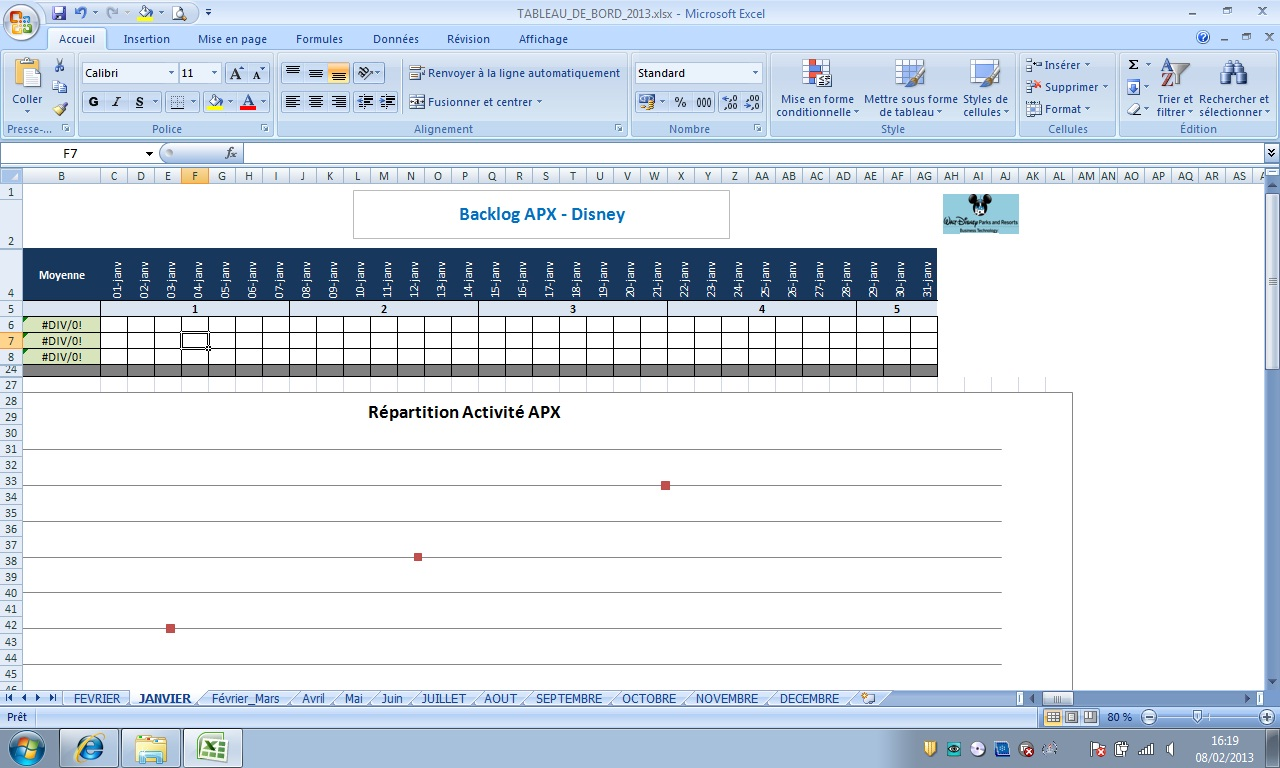
\includegraphics [width=1\textwidth]{images/tableauBordVide.jpg}
  \end{figure}
\end{center}
\begin{center}
  \begin{figure}[ht]
    \caption{\label{TabBordRempli} Tableau de bord après modifications de la macro"}
    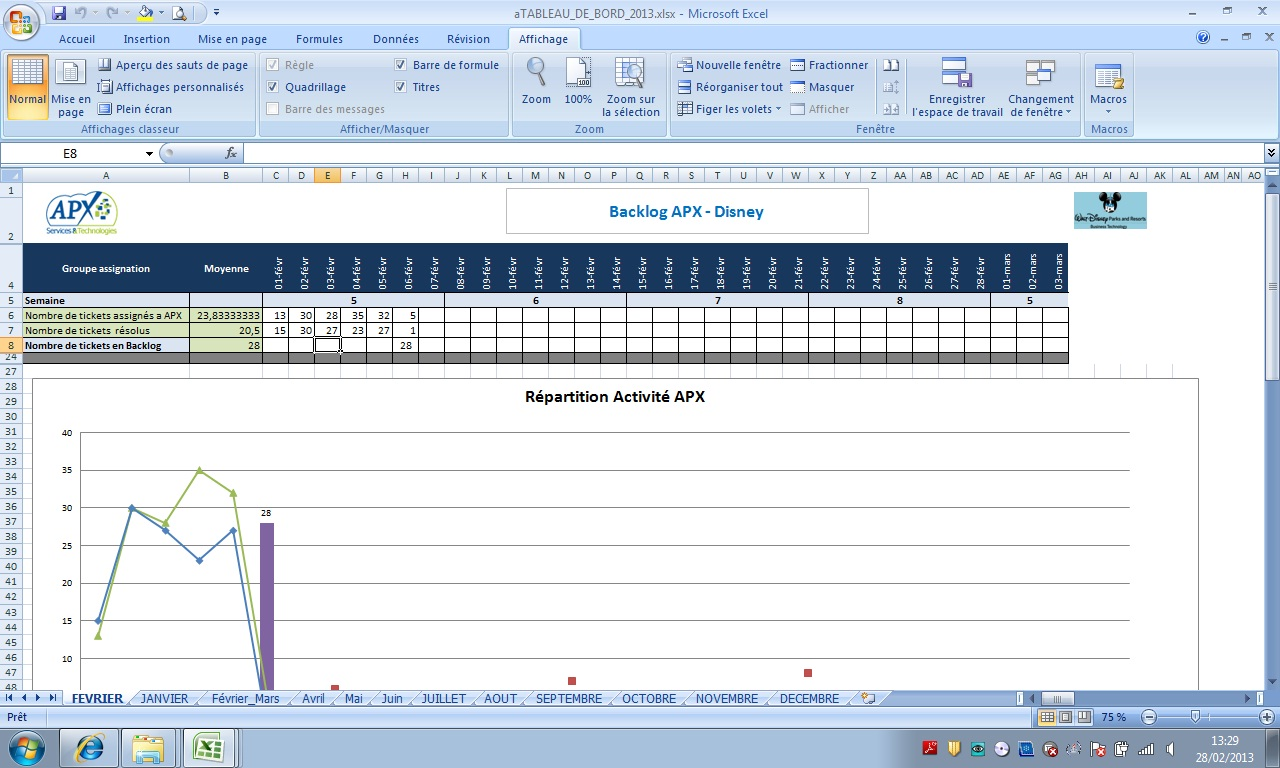
\includegraphics [width=1\textwidth]{images/TabBordRempli.jpg}
  \end{figure}
\end{center}

%listes
Enfin, mes dernières macros ont été plus simple à réaliser, il s'agissait le lister les interventions résolues et en \gls{backlog} avec quelques détails sur l'intervention (cf. figure~\ref{listeResolu} page~\pageref{listeResolu} et figure~\ref{listeBacklog} page~\pageref{listeBacklog}).



\subsection{La mise en production}%
\paragraph{}
Enfin, je voulais vous parler de la mise en production qui à été révélatrice de nombreux problèmes sur les statistiques avant la création de ces macros.
En effet, avant l'automatisation de ces tâches, les données utilisées étaient souvent les \gls{ri} papiers. Or dans certains cas, les \gls{ot} de ces \gls{ri} ont été transférés à un autre service ou bien annulés, mais ils comptais quand même dans nos statistique. Nos statistiques étaient donc faussées.
Avec la création de ces macros, les \gls{ot} annulés ou transférés ne sont pas comptés dans nos statistiques. De plus la feuille issue de la macro de "contrôle" permet de s'en assurer.
J'ai également créé une documentation afin que toutes les étapes nécessaires au bon fonctionnement des macros ne soient pas oubliés. En effet certaines options doivent être cochés dans Excel sans quoi les macros ne peuvent pas êtres lancées par exemple.

\paragraph{}
\newglossaryentry{launcher}{name={\foreignlanguage{english}{launcher}},description={Lanceur}}
Finalement, après de nombreux essais la mise en production de ces macros à été facilitée grâce à une dernière macro. Une macro qui fait office de "\foreignlanguage{english}{\gls{launcher}}\footnote{Lanceur}" de macros. 
J'ai donc crée une petite boite de dialogue où l'utilisateur peut saisir le nom des fichiers à modifier (le tableau de bord, le tableau de productivité des techniciens, etc...) et enfin lancer les macros les unes à la suite des autres (cf. figure~\ref{Launcher} page~\pageref{Launcher} et figure~\ref{nomDesFichiersAEditer} page~\pageref{nomDesFichiersAEditer}).
\begin{center}
  \begin{figure}[ht]
    \caption{\label{Launcher} Launcher de macros"}
    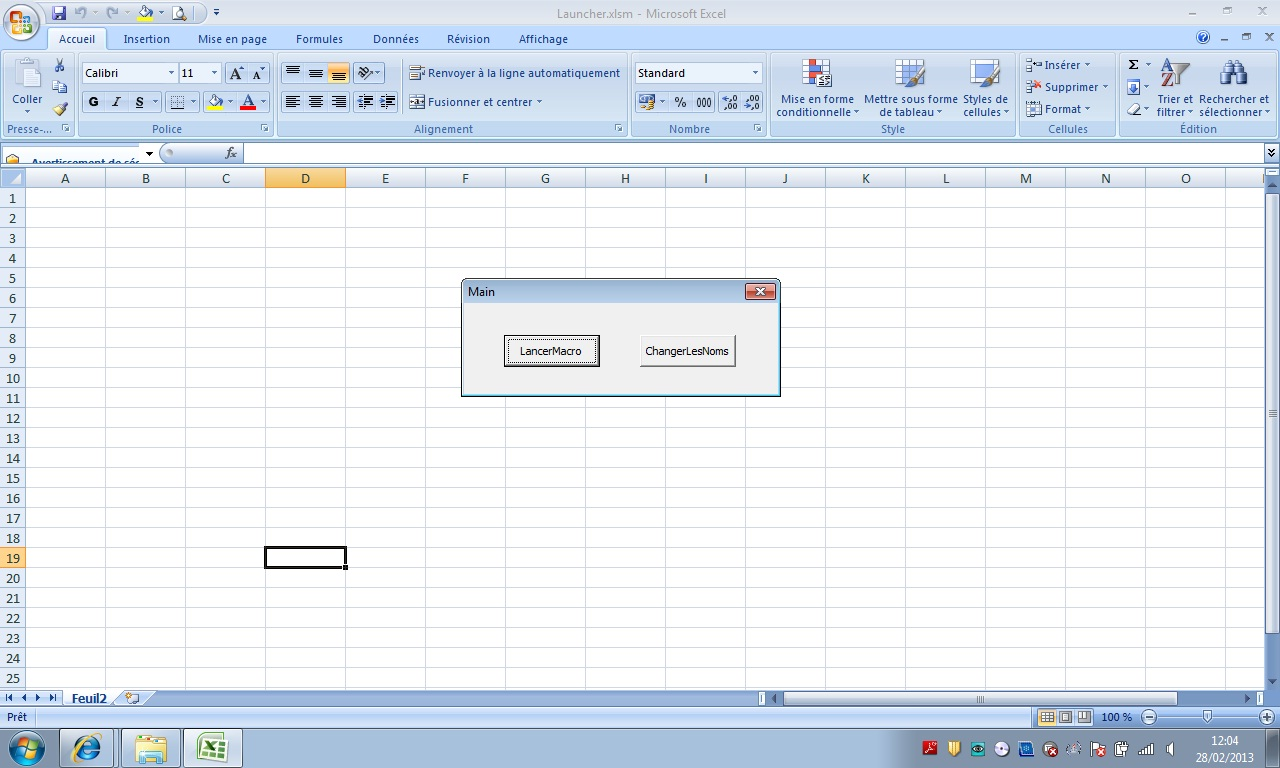
\includegraphics [width=1\textwidth]{images/Launcher.jpg}
  \end{figure}
\end{center}
\begin{center}
  \begin{figure}[ht]
    \caption{\label{nomDesFichiersAEditer} Changement des noms de fichiers dans le launcher"}
    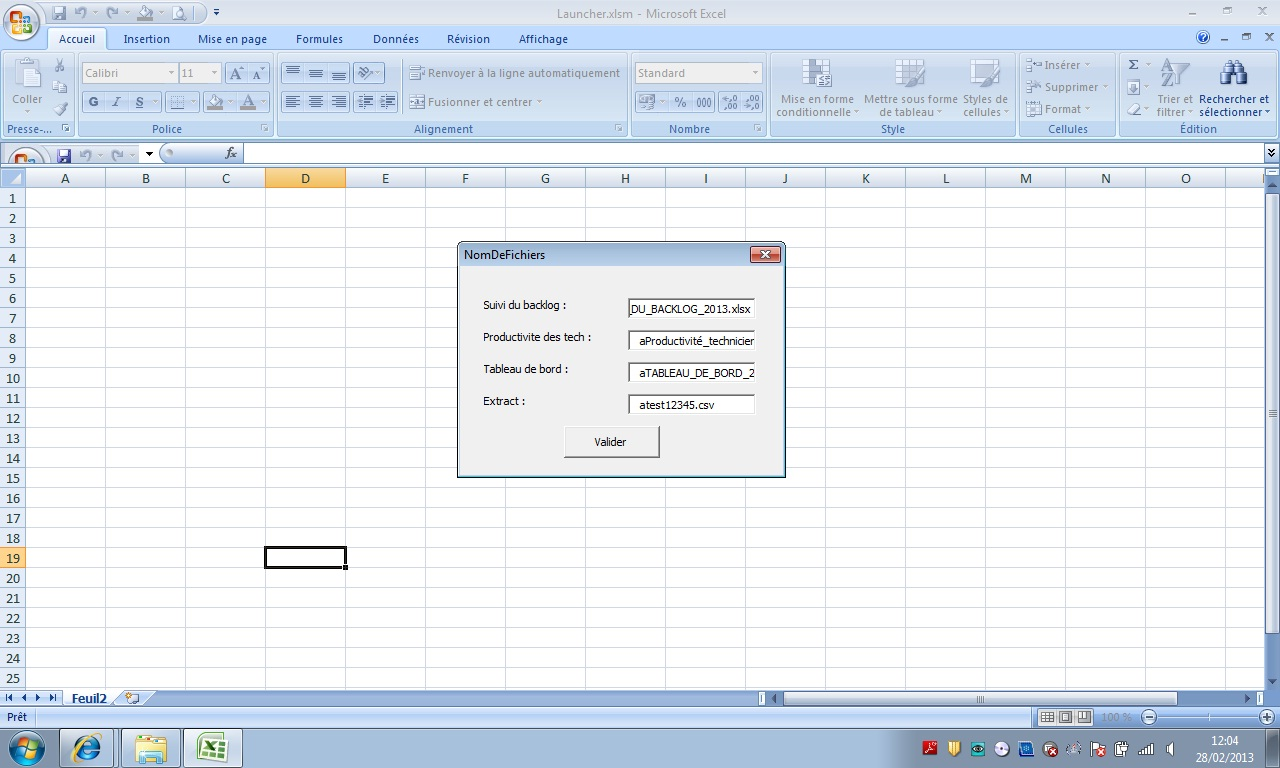
\includegraphics [width=1\textwidth]{images/nomDesFichiersAEditer.jpg}
  \end{figure}
\end{center}
